\documentclass{article}
\usepackage[nonatbib, preprint]{neurips_2023}

\usepackage[utf8]{inputenc}
\usepackage[T1]{fontenc}
\usepackage{hyperref}
\usepackage{url}
\usepackage{booktabs}
\usepackage{microtype}
\usepackage{xcolor}
\usepackage{subcaption}
\usepackage{xspace}
\usepackage{graphicx}
\usepackage{float}
\usepackage[backend=biber,style=numeric]{biblatex}

\bibliography{bibliography.bib}
\hypersetup{
  colorlinks=true,
  pdfencoding=auto,
  psdextra,
  pdfauthor={Luis Hagenauer, Laura Lavezza, Melih Mutlu},
  pdftitle={Analyzing the impact of Thanksgiving on the road accident frequency}
}

\title{Analyzing the impact of Thanksgiving on the road accident frequency}

\author{%
  Luis Hagenauer \\
  Matrikelnummer 5484904 \\
  \And
  Laura Lavezza \\
  Matrikelnummer 6737032 \\
  \And
  Melih Mutlu \\
  Matrikelnummer 6070834
}

\begin{document}
\maketitle

\begin{abstract}
  We analyze the frequency of road accidents in \emph{Montgomery County,
  Maryland, USA} and the impact of Thanksgiving on the number of accidents on
  the following days. In particular, by considering data from 2021-2024, we
  present significant evidence that the number of accidents on Thanksgiving is
  lower than usual and that the number of accidents on the three preceding days
  is higher than usual. These results were obtained by conducting Mann-Whitney U
  tests.
\end{abstract}

\section{Introduction}\label{sec:introduction}
Thanksgiving each year marks the fourth Thursday of November and can arguably be
considered the most relevant US-American public holiday. Holidays like
Thanksgiving are traditionally associated with increased traffic as individuals
travel to gather with family and friends. This surge in travel, combined with
increased celebratory activities and alcohol consumption, potentially escalates
the risk of road accidents. Understanding the relationship between holiday
events and accident frequency is crucial for developing targeted interventions.

This study aims to provide empirical evidence that could help develop policies
and safety strategies, ultimately enhancing road safety during periods of high
travel risk. We employ statistical analysis, particularly the Mann-Whitney U
test, to examine the assertion that the number of road accidents significantly
increases before Thanksgiving compared to non-holiday periods and decreases on
Thanksgiving Day itself.

With a total population of approximately one million, Montgomery County is the
most populous county in the state of Maryland, USA, and occupies an area of
about 1,300 km$^2$.  The diversity of urban infrastructure that characterizes
Montgomery County, along with the large volume of available data, makes the
region well-suited for the purposes of this study.

\section{Dataset and cleaning process}
The raw data was downloaded from the Montgomery County data catalog
\cite{dataset} in the form of a CSV table which contains a total number of
190824 data points (rows) and 39 features (columns). To ensure consistency and
improve readability, the column names were normalized and the one containing
information about the date and time of the crash was divided into the columns
\emph{year}, \emph{month}, \emph{day}, \emph{time}. Although the dataset did not
show any duplicates, several columns reported a significant percentage of
missing values. In particular, five columns presented a percentage higher than
80\%, leading to the decision to drop these features as they would not be useful
for any exploratory analysis.

\section{Exploratory data analysis and preprocessing}
\subsection{Baseline definition for data analysis}
To make meaningful statements about systematic increase or decrease of the
Number of Accidents (NoA), we need to specify an appropriate baseline for the
analysis. Thus, we want to find a suitable subset of the data, that is, its data
points were collected under similar conditions and follow the same distribution.
In addition, we have to design a sound stochastic model to apply statistical
methods.

Our analysis suggests that the NoA per day depends both on year (see
Fig.~\ref{fig:accidents_per_year}) and month (see
Fig.~\ref{fig:accidents_per_month}). In particular, it appears as if the
distribution of NoA per year is different between period 2015-2019 and
2021-2024. This trend could be attributed to the global COVID pandemic starting
in early 2020 and the accompanying increase in remote work \cite{workfromhome}.
This study focuses on the period 2021-2024. Even though this comes with the
limitation of having fewer data points available compared to the first period,
it frees us from considering possible external factors that might be difficult
to take into account. Examples of such elements could be changes in the general
behavior of drivers before and after pandemic or in the way road accidents are
reported.

Regarding the distribution over the months, we observe similarity in terms of
NoA for the fall/winter months of October, November and December. The similarity
might be due to similar external factors, such as weather conditions. Therefore,
we then define our baseline or \emph{reference period} as the data from the
months October-December of the years 2021-2024.

\begin{figure}[H]
  \centering
  \begin{minipage}[t]{0.45\textwidth}
    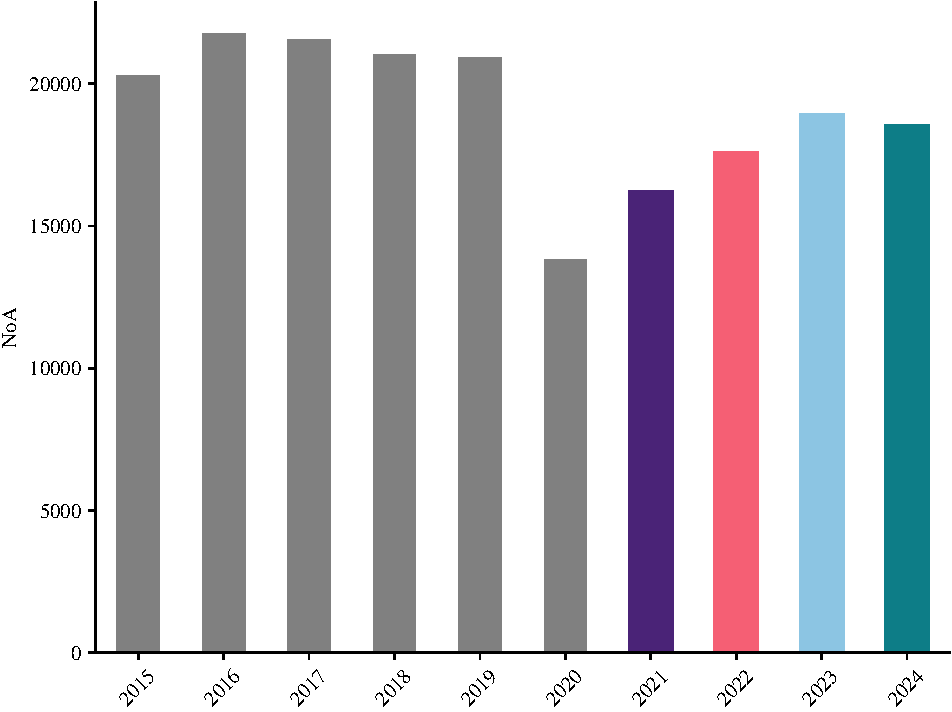
\includegraphics[width=\textwidth]{../fig/accidents_per_year.pdf}
    \caption{NoA per year}\label{fig:accidents_per_year}
  \end{minipage}
  \hspace{0.5cm}
  \begin{minipage}[t]{0.45\textwidth}
    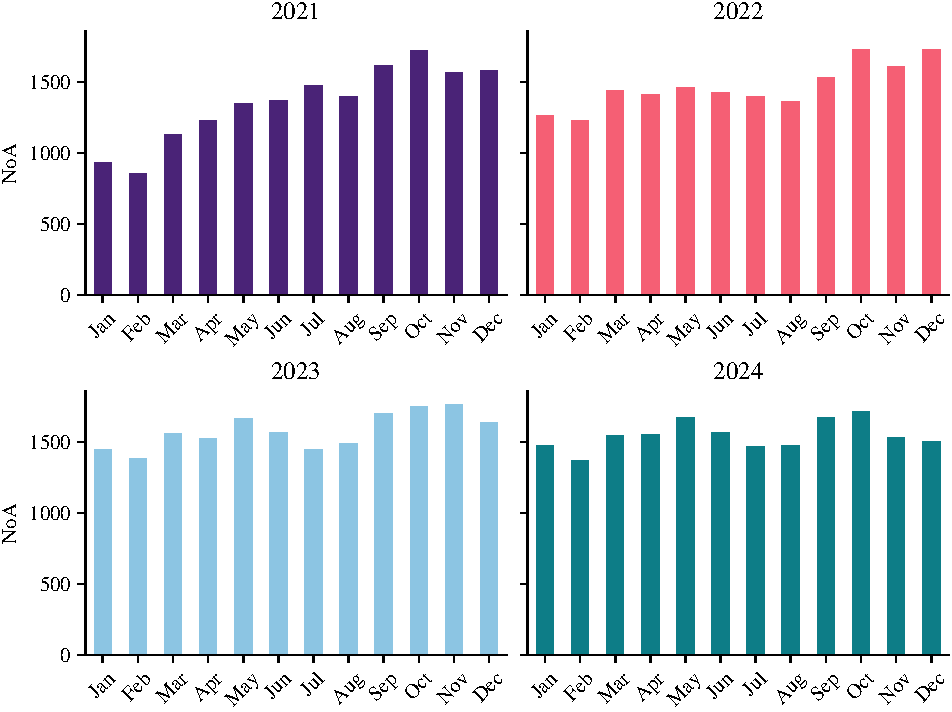
\includegraphics[width=\textwidth]{../fig/accidents_per_month.pdf}
    \caption{NoA per month}\label{fig:accidents_per_month}
  \end{minipage}
\end{figure}

\subsection{Accident patterns in the month of Thanksgiving}
Since we are particularly interested in studying the impact of Thanksgiving on
the frequency of road accidents, we searched for possible patterns in November
for the years of the reference period. This investigation outlined a significant
drop in the NoA on Thanksgiving, while an increase was registered around three
days before (see Fig.~\ref{fig:accidents_per_day}).
\begin{figure}[H]
  \centering
    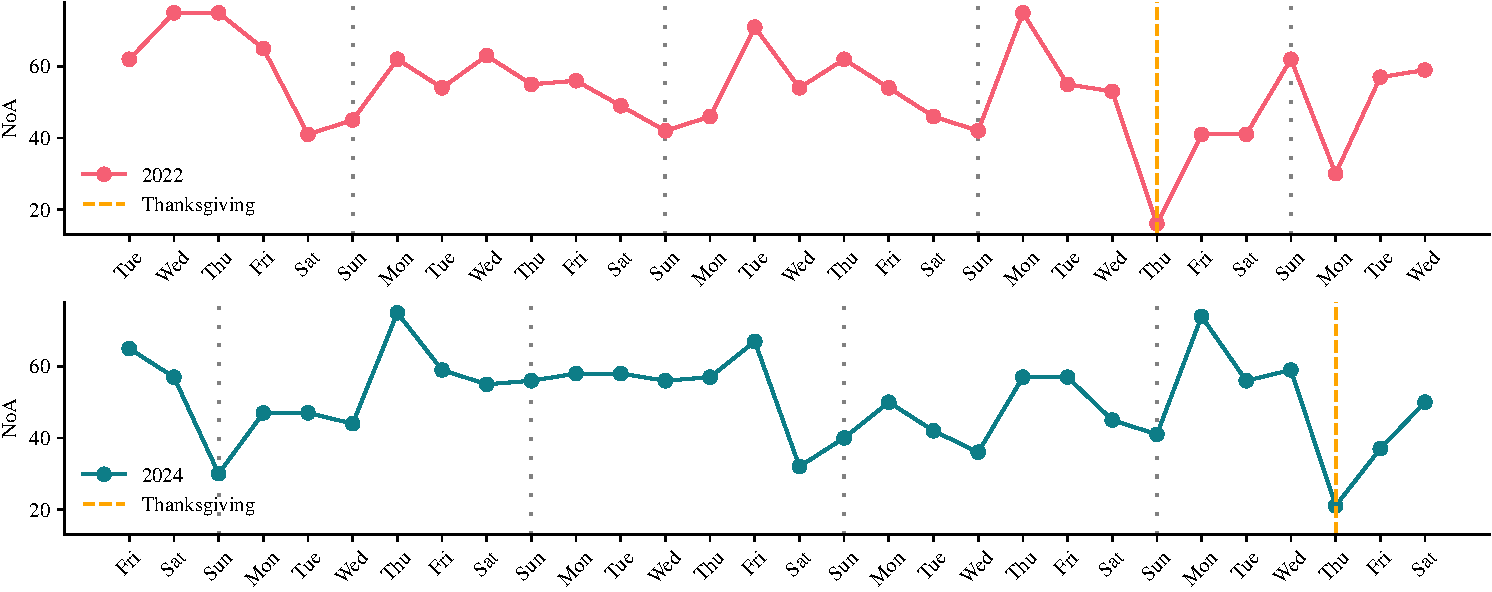
\includegraphics[height=5cm]{../fig/accidents_per_day.pdf}
    \caption{NoA in November}\label{fig:accidents_per_day}
\end{figure}

\subsection{Accident patterns on the days of the week}\label{sec:noa_day_of_week}
\begin{figure}[H]
  \begin{minipage}{0.4\textwidth}
    Given the visible effect of weekends on the NoA (see
    Fig.~\ref{fig:accidents_per_day}) for the month of November, we need to
    verify that this influence is also present in the other months of the reference
    period. This indeed appears to be the case (see
    Fig.~\ref{fig:accidents_per_day_of_week}). Therefore, to correctly apply our
    statistical model we need to group data points by day of the week. Otherwise we
    would have data coming from different distributions which would bias our
    analysis.
  \end{minipage}
  \hspace{0.02\textwidth}
  \raisebox{-.7cm}[0pt][0pt]{
    \begin{minipage}{0.6\textwidth}
      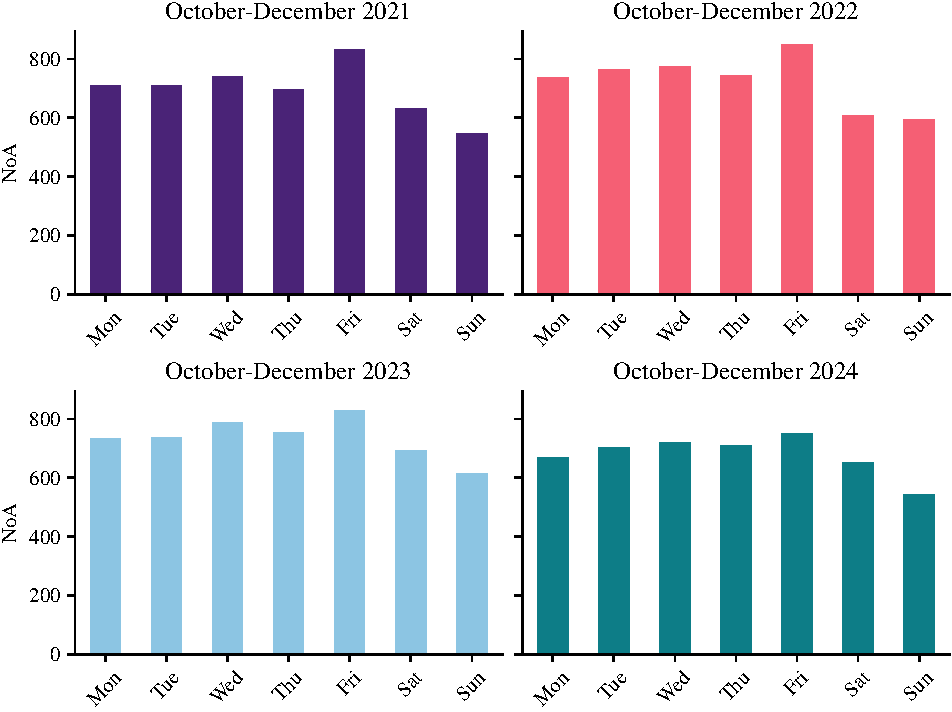
\includegraphics[width=0.9\textwidth]{../fig/accidents_per_day_of_week.pdf}
      \caption{NoA per day of week}\label{fig:accidents_per_day_of_week}
    \end{minipage}
  }
\end{figure}

\vspace{1cm}

\subsection{Statistical model}
We assume that the NoA on each day in the reference period is independent and
furthermore that each separate day of the week follows the same distribution,
i.\,e.\xspace all Mondays are iid. In particular, this assumption allows us to
consider data points from one day of the week as samples drawn from an unknown
distribution. See Section~\ref{sec:discussion} for the limitations that lie with
these assumptions.

A common approach would be to assume that the NoA per day (grouped by day of
week) is normally distributed. However, the long tail and lack of symmetry in
the observed data (see Fig.~\ref{fig:accidents_on_thursdays}) did not allow to
comfortably rely on normality.

\begin{figure}[H]
  \centering
  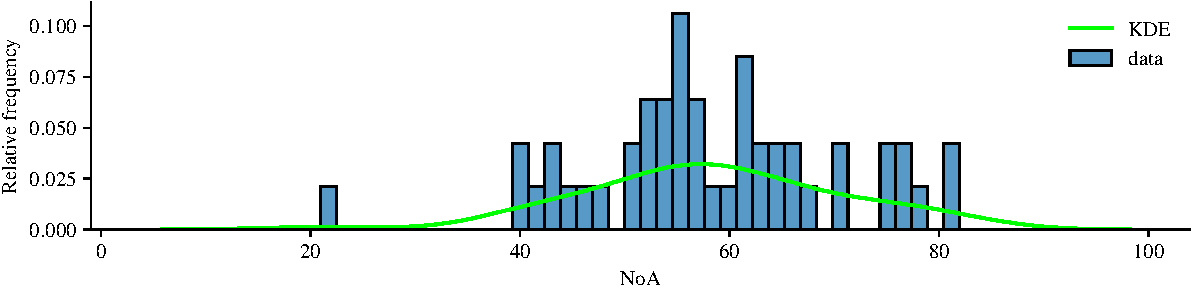
\includegraphics[width=\textwidth]{../fig/accidents_on_thursdays.pdf}
  \caption{Relative histogram of NoA on Thursdays during
  reference period; kernel density estimate (KDE) using Gaussian smoothing}
  \label{fig:accidents_on_thursdays}
\end{figure}

\section{Testing of hypotheses and results}
Taking into account the consideration in the previous section, we decided to use
the (nonparametric) Mann-Whitney U test with a level of significance of 5\%. We
conduct separate tests for the following alternative hypotheses:
\begin{itemize}
  \item NoA on Thanksgiving is \emph{less} compared to usual days.
  \item NoA on Monday before Thanksgiving is \emph{greater} compared to usual
    days.
  \item NoA on Tuesday before Thanksgiving is \emph{greater} compared to usual
    days.
  \item NoA on Wednesday before Thanksgiving is \emph{greater} compared to usual
    days.
  \item Aggregated NoA on Monday, Tuesday and Wednesday before Thanksgiving is
    \emph{greater} compared to usual days.
\end{itemize}

\pagebreak
For each testing procedure, call days in the reference period \emph{usual} if
\begin{itemize}
  \item they are not the days in the claim,
  \item they are on the same day of week as the days in the claim (see Section~\ref{sec:noa_day_of_week}),
  \item they are not part of the blocklist consisting of October 14th, December
    25th and December 31st.
\end{itemize}
For instance, for the first test we consider all Thursdays in the reference
period and exclude Thanksgiving day as well as the blocklist from our baseline
data. This is done so that we do not compare days to themselves and to avoid the
inclusion of "special" days like Christmas or Silvester.

Summarizing the test results in Table~\ref{tab:results}, we have significant
evidence that the NoA on Thanksgiving day is indeed lower compared to usual
days. Additionally, the aggregated NoA on the three preceding days is elevated.

\begin{table}[H]
  \centering
  \begin{tabular}{c c c c c}
    \toprule
    & $H_1$ & $U$ & p-value & reject $H_0$ \\
    \midrule
    Thanksgiving & less & 2.5 & 0.000711 & yes \\
    Mon before & greater & 155.0 & 0.012564 & yes \\
    Tue before & greater & 142.5 & 0.056827 & no \\
    Wed before & greater & 100.5 & 0.596969 & no \\
    Mon, Tue, Wed before aggregated & greater & 172.0 & 0.006657 & yes \\
    \bottomrule
  \end{tabular}
  \caption{Results for Mann-Whitney U tests}\label{tab:results}
\end{table}
\section{Discussion}\label{sec:discussion}
As a consequence of this study, we are indeed confident that the number of road
accidents significantly decreases on Thanksgiving Day. However, we cannot
conclude a systematic increase for the three single days before Thanksgiving but
only for the aggregation of these days.

Interpreting our results, it is important to consider several limitations.
Firstly, our inclusion of days in the blocklist is best-effort and in that sense
rather arbitrary. We do not take other potential special events (such as sports
games) into account. Moreover, we assumed independence of the NoA on each day in
the reference period but it is imaginable that people drive more carefully
because of a high NoA on the previous day. The assumption of identical
distribution could also possibly be violated by extreme weather events that
cause a spike in the NoA. By merely using the present data, it is relatively
difficult to statistically determine whether this is \emph{not} the case.

\section{Statement of Contributions}
MM took care of finding the dataset for our task, taking into consideration the
necessary features and data availability. LL performed data cleaning and
normalization. All members were responsible for the exploratory data analysis.
LH designed the statistical model and conducted the tests to verify our
hypotheses. LL and LH produced the plots for this report and restructured the
pipeline for the data analysis. All members of the group contributed to writing
the report and MM proof-read the draft for the final report.
\printbibliography
\end{document}
